% Created 2019-10-13 Вс 22:46
% Intended LaTeX compiler: pdflatex
\documentclass[11pt]{article}
\usepackage{lscape}
\usepackage[utf8]{inputenc}
\usepackage[T1]{fontenc}
\usepackage{graphicx}
\usepackage{grffile}
\usepackage{longtable}
\usepackage{graphicx}
\usepackage{wrapfig}
\usepackage{rotating}
\usepackage[normalem]{ulem}
\usepackage{amsmath}
\usepackage{textcomp}
\usepackage{amssymb}
\usepackage{capt-of}
\usepackage{hyperref}
\usepackage[T2A]{fontenc}
\usepackage[a4paper,left=3cm,top=2cm,right=1.5cm,bottom=2cm,marginparsep=7pt,marginparwidth=.6in]{geometry}
\usepackage{cmap}
\usepackage[russian]{babel}
\usepackage{xcolor}
\usepackage{color}
\usepackage{listings}
\definecolor{pblue}{rgb}{0.13,0.13,1}
\definecolor{pgreen}{rgb}{0,0.5,0}
\definecolor{pred}{rgb}{0.9,0,0}
\definecolor{pgrey}{rgb}{0.46,0.45,0.48}
\usepackage{listings}
\lstset{extendedchars=\true,
	language=Java,
	showspaces=false,
	showtabs=false,
	breaklines=true,
	showstringspaces=false,
	breakatwhitespace=true,
	commentstyle=\color{pgreen},
	keywordstyle=\color{pblue},
	stringstyle=\color{pred},
	basicstyle=\ttfamily,
	moredelim=[il][\textcolor{pgrey}]{$$},
	moredelim=[is][\textcolor{pgrey}]{\%\%}{\%\%}
}
\author{АВТОР}
\date{\today}
\title{}
\hypersetup{
 pdfauthor={АВТОР},
 pdftitle={},
 pdfkeywords={},
 pdfsubject={},
 pdfcreator={Emacs 26.1 (Org mode 9.1.9)}, 
 pdflang={Russian}}
\begin{document}

\large
\thispagestyle{empty}
\begin{center}
\textbf{Национальный Исследовательский Университет ИТМО}\\
\textbf{Факультет Программной Инженерии и Компьютерной Техники}\\
\end{center}
\vspace{2em}
\begin{center}

\includegraphics[width=120px]{../../../itmo-logo.png}
\end{center}
\LARGE
\vspace{5em}
\begin{center}
\textbf{Вариант № 82002}\\
\textbf{Лабораторная работа № 2}\\
\Large
\textbf{по дисциплине}\\
\LARGE
\textbf{\emph{'Программирование'}}\\
\end{center}
\vspace{11em}
\large
\begin{flushright}
\textbf{Выполнил:}\\
\textbf{Студент группы P3113}\\
\textbf{\emph{Куперштейн Дмитрий;} : 269359}\\
\textbf{Преподаватель:}\\
\textbf{\emph{ПИСЬМАК АЛЕКСЕЙ ЕВГЕНЬЕВИЧ}}\\
\end{flushright}
\vspace{4em}
\large
\begin{center}
\textbf{Санкт-Петербург 2019 г.}
\end{center}
\pagebreak{}
\setcounter{tocdepth}{2}
\tableofcontents
\vspace{2em}
\pagebreak
\section{Задание}
На основе базового класса \texttt{Pokemon} написать свои классы для заданных видов покемонов. Каждый вид покемона должен иметь один или два типа и стандартные базовые характеристики:
\begin{itemize}
	\item очки здоровья (HP)
	\item атака (attack)
	\item защита (defense)
	\item специальная атака (special attack)
	\item специальная защита (special defense)
	\item скорость (speed)
\end{itemize}
Классы покемонов должны наследоваться в соответствии с цепочкой эволюции покемонов. На основе базовых классов \texttt{PhysicalMove}, \texttt{SpecialMove} и \texttt{StatusMove} реализовать свои классы для заданных видов атак.\\
Используя класс симуляции боя \texttt{Battle}, создать 2 команды покемонов (каждый покемон должен иметь имя) и запустить бой.\\
Базовые классы и симулятор сражения находятся в jar-архиве \texttt{Pokemon.jar} (обновлен 9.10.2018, исправлен баг с добавлением атак и кодировкой). 
Документация в формате javadoc -- \texttt{https://se.ifmo.ru/\~{}tony/doc/}.\\\\
Покемоны для варианта 82002:\\\\
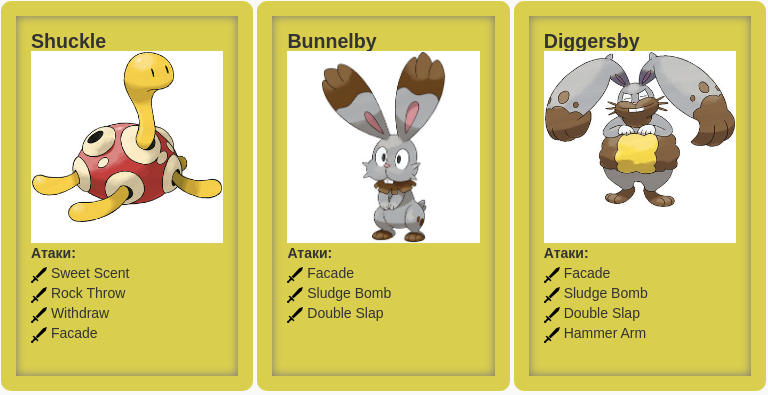
\includegraphics[width=250px]{../cards.png}\\
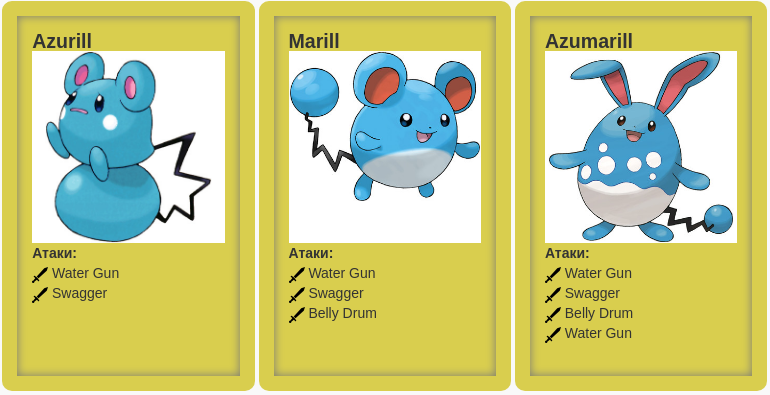
\includegraphics[width=250px]{../cards1.png}
\pagebreak
\section{Диаграмма классов реализованной объектной модели}
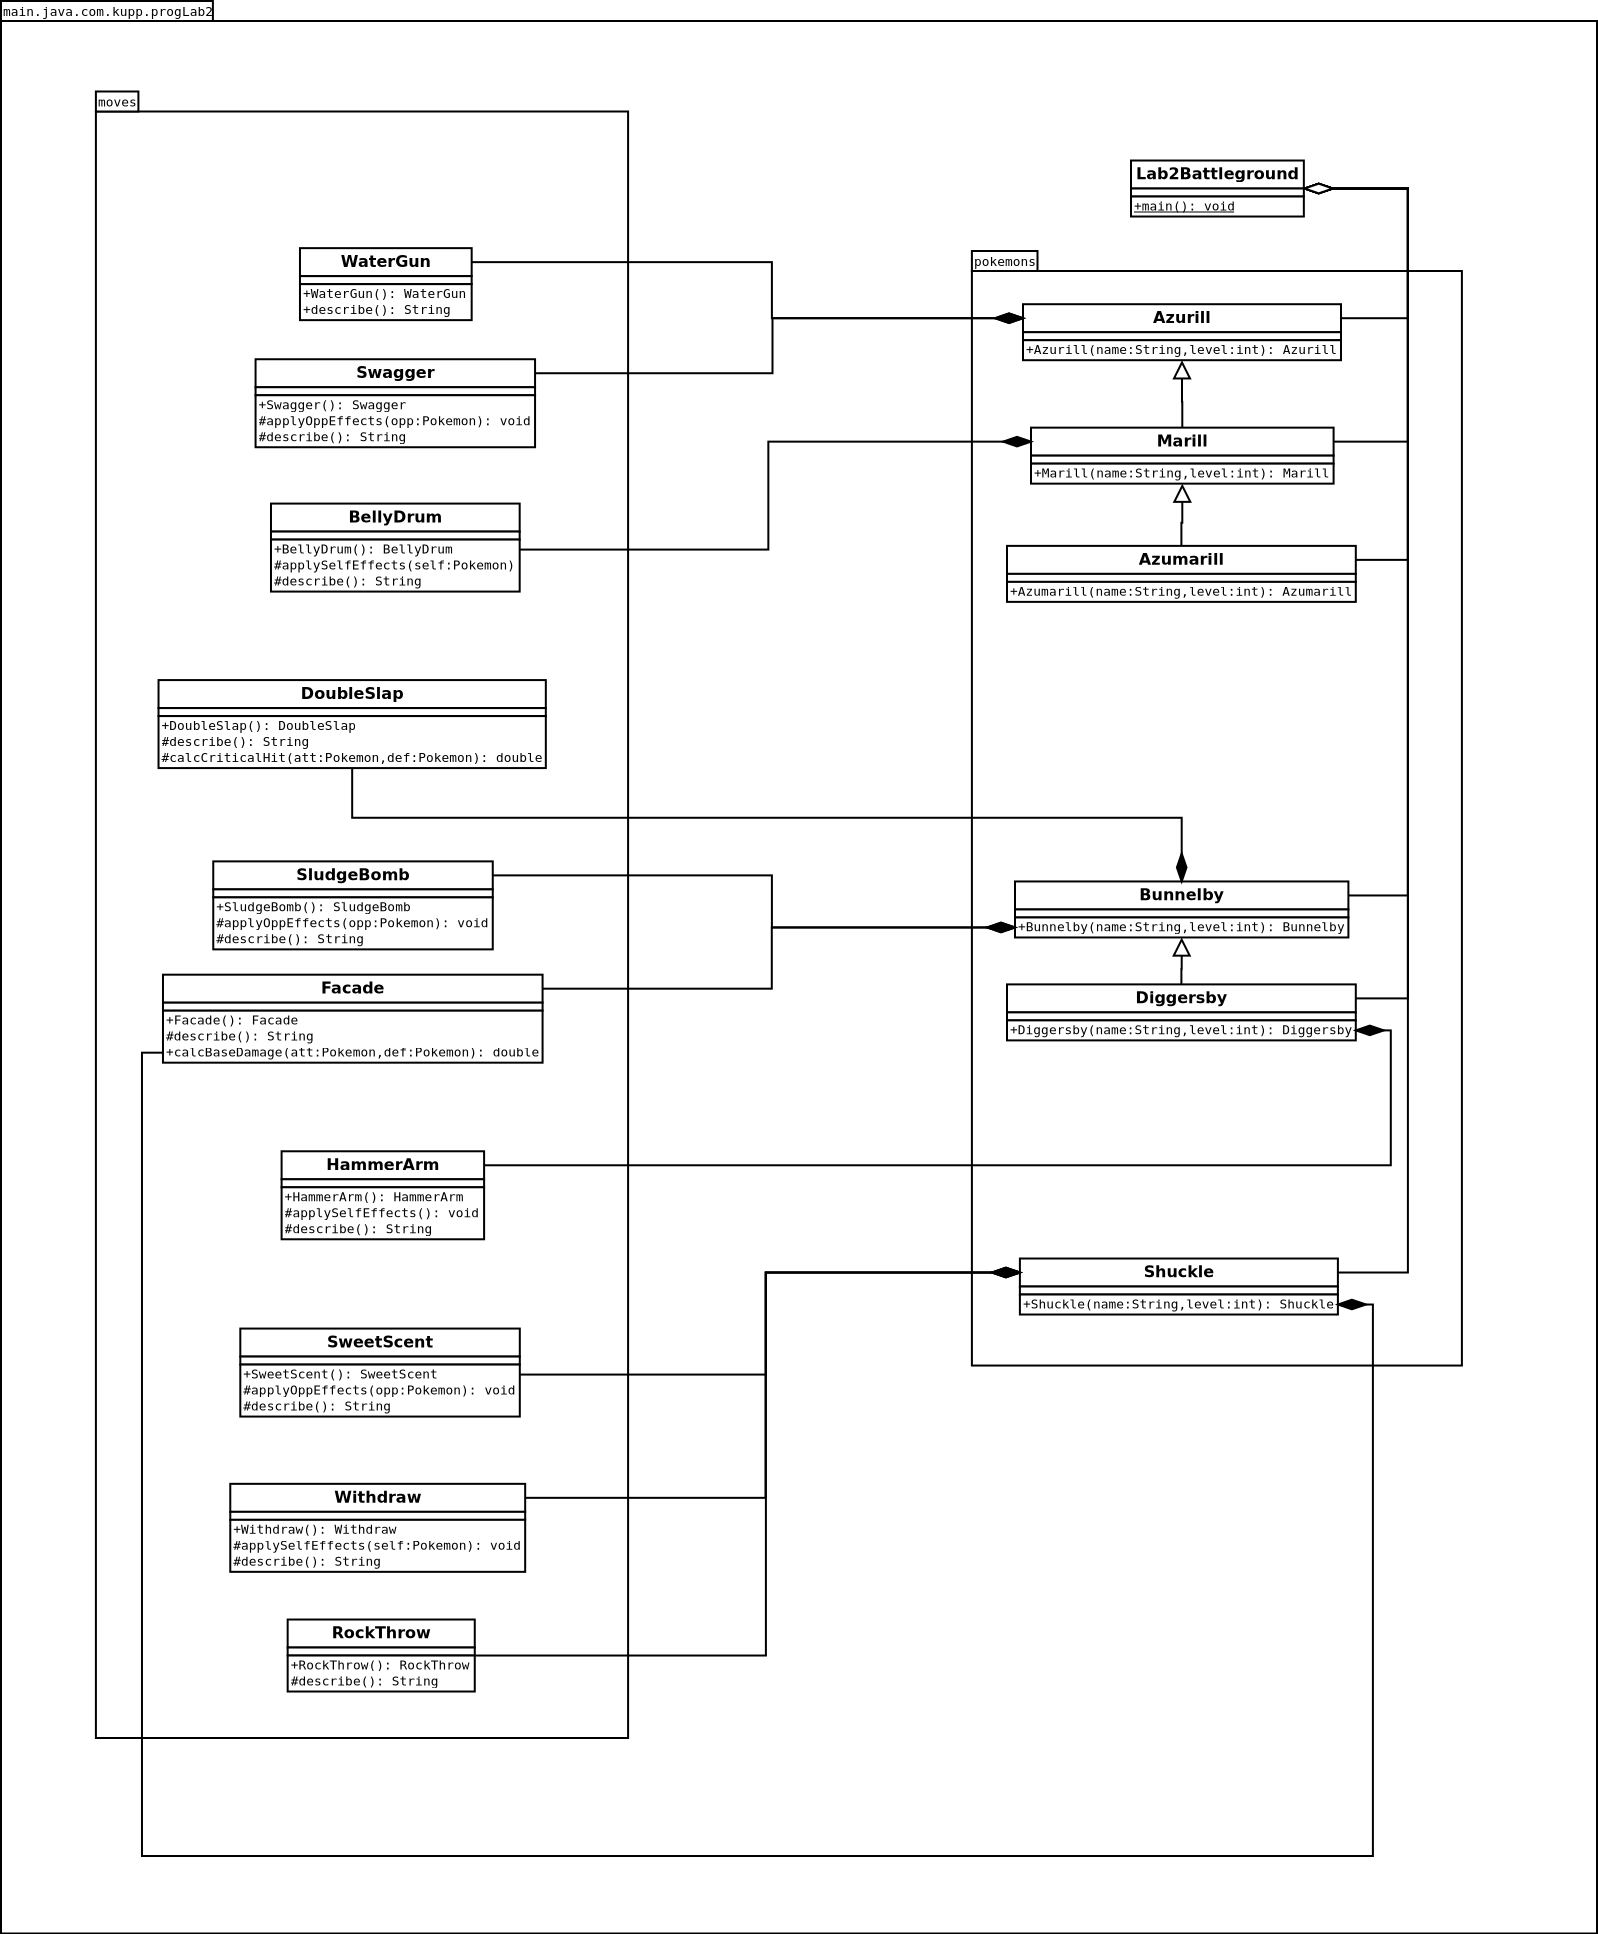
\includegraphics[width=500px]{../Diagram1.png}
\pagebreak
\section{Исходный код программы}
\small
\subsection{\texttt{main.java.com.kupp.progLab2}}
\subsubsection{Lab2Battleground.java}
\lstinputlisting[numbers=left, language=java]{../PokemonLab/src/main/java/com/kupp/progLab2/Lab2Battleground.java}
\subsection{\texttt{main.java.com.kupp.progLab2.moves}}
\subsubsection{BellyDrum.java}
\lstinputlisting[numbers=left, language=java]{../PokemonLab/src/main/java/com/kupp/progLab2/moves/BellyDrum.java}
\pagebreak
\subsubsection{DoubleSlap.java}
\lstinputlisting[numbers=left, language=java]{../PokemonLab/src/main/java/com/kupp/progLab2/moves/DoubleSlap.java}
\subsubsection{Facade.java}
\lstinputlisting[numbers=left, language=java]{../PokemonLab/src/main/java/com/kupp/progLab2/moves/Facade.java}
\subsubsection{HammerArm.java}
\lstinputlisting[numbers=left, language=java]{../PokemonLab/src/main/java/com/kupp/progLab2/moves/HammerArm.java}
\subsubsection{RockThrow.java}
\lstinputlisting[numbers=left, language=java]{../PokemonLab/src/main/java/com/kupp/progLab2/moves/RockThrow.java}
\pagebreak
\subsubsection{SludgeBomb.java}
\lstinputlisting[numbers=left, language=java]{../PokemonLab/src/main/java/com/kupp/progLab2/moves/SludgeBomb.java}
\subsubsection{Swagger.java}
\lstinputlisting[numbers=left, language=java]{../PokemonLab/src/main/java/com/kupp/progLab2/moves/Swagger.java}
\subsubsection{SweetScent.java}
\lstinputlisting[numbers=left, language=java]{../PokemonLab/src/main/java/com/kupp/progLab2/moves/SweetScent.java}
\subsubsection{WaterGun.java}
\lstinputlisting[numbers=left, language=java]{../PokemonLab/src/main/java/com/kupp/progLab2/moves/WaterGun.java}
\subsubsection{Withdraw.java}
\lstinputlisting[numbers=left, language=java]{../PokemonLab/src/main/java/com/kupp/progLab2/moves/Withdraw.java}
\pagebreak
\subsection{\texttt{main.java.com.kupp.progLab2.pokemons}}
\subsubsection{Azurill.java}
\lstinputlisting[numbers=left, language=java]{../PokemonLab/src/main/java/com/kupp/progLab2/pokemons/Azurill.java}
\subsubsection{Marill.java}
\lstinputlisting[numbers=left, language=java]{../PokemonLab/src/main/java/com/kupp/progLab2/pokemons/Marill.java}
\subsubsection{Azumarill.java}
\lstinputlisting[numbers=left, language=java]{../PokemonLab/src/main/java/com/kupp/progLab2/pokemons/Azumarill.java}
\pagebreak
\subsubsection{Bunnelby.java}
\lstinputlisting[numbers=left, language=java]{../PokemonLab/src/main/java/com/kupp/progLab2/pokemons/Bunnelby.java}
\subsubsection{Diggersby.java}
\lstinputlisting[numbers=left, language=java]{../PokemonLab/src/main/java/com/kupp/progLab2/pokemons/Diggersby.java}
\subsubsection{Shuckle.java}
\lstinputlisting[numbers=left, language=java]{../PokemonLab/src/main/java/com/kupp/progLab2/pokemons/Shuckle.java}
\section{Результат работы программы}
\lstinputlisting[numbers=left, language=]{../sample_out.txt}
\large
\section{Вывод}
В ходе этой лабораторной работы я поработал с документацией к классу Pokemon и реализовал на его основе заданных покемонов и заданные атаки, как следствие поработал с ООП в Java.

\end{document}